\section{Methodology}\label{Sec:AdditionalMethodology}


\subsection{Preregistration and data}
This study's methodology, data collection procedures, sample size, exclusion criteria, and hypotheses were preregistered on the Open Science Framework (OSF) in advance of the data collection and analysis. The preregistration can be accessed at \url{https://osf.io/mgex3}, while the obtained data and the experiment played by the participants is available at \url{https://osf.io/gtuwp/}.

In this work we also make some exploratory (not preregistered) analyses: we correct for verbal explanations that are not consistent with a positive interpretation of the concept for Hypothesis~\ref{Hip:AndOverOr}, we exclude outliers from the analysis in Hypothesis~\ref{Hip:FeatureBiasTimeAdvantage}, and we consider the effect of the participant's learning history  beyond the immediately previous trial in Hypothesis~\ref{Hip:FeatureBiasStickiness}. We also explicitly analyse, in this framework of multiple consistent explanations, the difference in revealed difficulty between rules of greatly differing minimal length.


\subsection{Representational details}\label{sub:experimentdetails} 


The underlying mathematical structure of the trials uses propositional variables, valuations, and sets of valuations. However, these are not shown abstractly, but rather are represented via correspondences to features (symbols), elements (boxes), and concepts (collections of elements). 

We next describe details of the representations used for the experiment and its competing concepts.


\paragraph{Features\textemdash propositional variables}
The experiment encompasses eight propositional variables: $p_1,\dots,p_8$. Each variable can take one of two possible values, and these values are graphically represented by icons. For instance, $p_1$ can be assigned icon `A' or icon `B', representing the values 1 (positive) and 0 (negative) respectively, $p_3$ can be assigned a `$+$' icon or `$\times$' icon  representing 1 and 0 respectively, and so on. 

Figure~\ref{Figure:references} shows the pairs of values for each of the eight propositional variables. The assignment of pairs of icons to propositional variables is randomized at the start of the experiment, and does not vary within the experiment. 
The reason to choose icons instead of (colored) values 0,1 is to avoid the possibility of mentally learning a concept using `counting' or other operators not present in propositional logic. For example, showing explicit $\{0,1\}$ values, a possible explanation for a concept could be {\em more than 3 ones}, but such a description would be much harder in the icon-based representation, since different propositional variables have no symbols in common. In \S\ref{Experiment_design} we discuss more details on these considerations.

\begin{figure}[h!]
\begin{center}
    	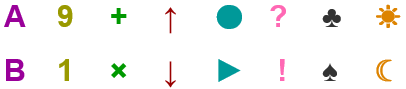
\includegraphics[scale=2]{Images/Features8.png}
	\caption{Pictured above are the features, the visual representation of the positive and negative values of the propositional variables. The upper row represents positive values of the propositional variables, while the lower row represents their negation.}
	 \label{Figure:references}
\end{center}
\end{figure}


\paragraph{Elements (boxes)\textemdash valuations.} A valuation over the propositional variables is visually represented as a square/box with the values (icons) of all propositional variables set at random positions inside the square. We call such representation an `element' (see Figure~\ref{Figure:element} for an example of such an element). The reason for choosing this representation is to avoid directional biases that could influence learning, and to exclude ordering and other operators from the language of thought (see \S\ref{Experiment_design} for more details). 
Each time an element is shown (in particular, within the loop in the training-feedback) a new random position is chosen for the propositional features inside it.
%

\begin{figure}[h!] 
\begin{center}
    	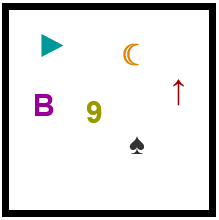
\includegraphics[scale=0.6]{Images/BordeNeutro.PNG}
	\caption{An element. This box containing features is the visual representation of a valuation over six propositional variables. Here the box appears with a neutral border, but boxes in the experiment always appear with a border that denotes whether they are positive or negative examples. The position of the symbols is irrelevant for the concepts, and is randomly assigned.}
	\label{Figure:element} 
\end{center}
\end{figure}


\paragraph{Undetermined concepts\textemdash sets of positive/negative valuations.}\label{IncompleteConcepts} The concept shown in the learning stage of a trial corresponds to two non-overlapping sets of valuations, and these two sets do not cover all possible valuations. This is represented as a sequence of `in' and `out' elements, with no information given on elements that are not shown. % (that does not show all possibilities). 
At the learning stage, shown `in' elements (positive examples) are represented as a green box and shown `out' elements (negative examples) as a red box. See Figure~\ref{Figure:training} for an example of a tagged sequence of elements used in the learning stage. Each time the concept is presented, we shuffle the order in which their positive and negative examples are shown, but always presenting all positive examples first (also, each valuation is assigned new random positions for the features inside the corresponding box). 

\begin{figure}[h!] 
\begin{center}
    	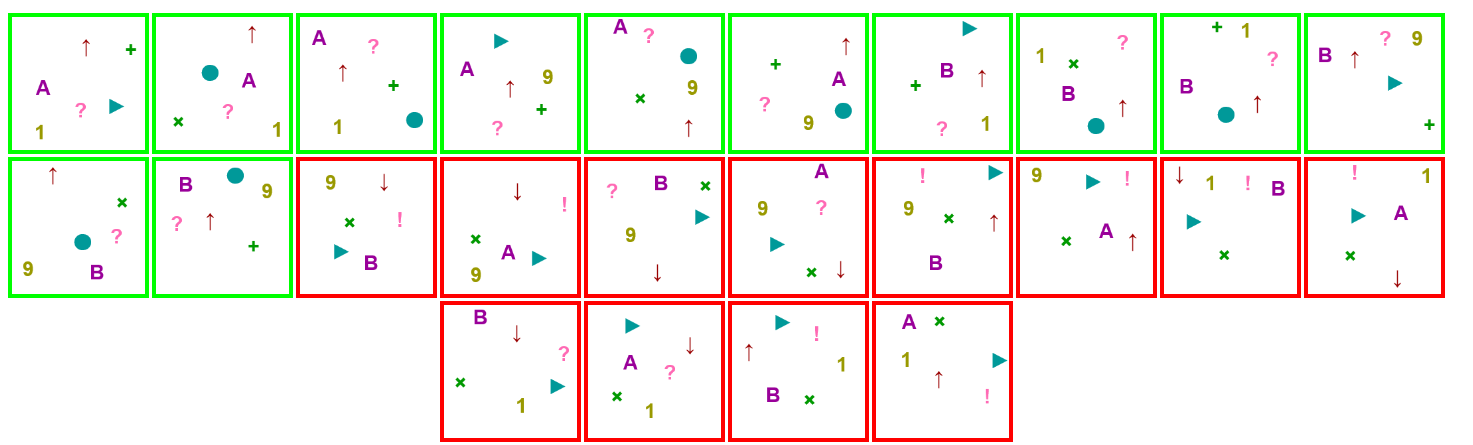
\includegraphics[scale=0.35]{Images/Learning.PNG}
	\caption{A sequence of positive and negative examples in a learning stage, corresponding to Trial 1.  A green border informs the participant that the element belongs to the concept, while a red-bordered one informs that it does not belong to the concept. In this case, the examples could be explained as either `boxes containing both an upwards pointing arrow and a question mark' or as `boxes that contain a circle or a plus sign', but note that these two rules determine different concepts over the complete set of possible elements.}
	\label{Figure:training}
\end{center}
\end{figure}

\paragraph{(Hidden) concepts\textemdash formulas.}
Over the full set of valuations, a concept is simply the set of valuations that positively describe it. The two hidden concepts for each trial correspond to the valid and minimal generalizations that can be made from the incomplete concepts. They can be described as the semantics of the two propositional formulas (rules) that can be used to explain the incomplete concept (see Table~\ref{trial_table}); while these rules coincide over the incomplete universe shown in the learning stage, they differ over the set of all valuations. For more details, recall the beginning of \S\ref{Subsec:ExperimentFlow} and its Item~\ref{item:LearningStage}. For technical details, see \S\ref{Sec:MainTheoremConcept}.

\bigskip

In Table~\ref{tab:glosario} we summarize the main logical terminology used to define formal semantics, and its representational counterpart adopted in our experimental setup.

\begin{table}[]
\begin{tabular}{c|c}
{\bf Mathematical terminology}
&
{\bf Representational terminology}
\\\hline
\begin{minipage}[t]{0.45\textwidth}
{\bf Valuation}: a tuple $\overline v=(v_1,\dots,v_n)$ where each $v_i$ is 0 or 1. 
\end{minipage}
& 
\begin{minipage}[t]{0.45\textwidth}
{\bf Element}: a square with $n$ symbols inside (see Figure~\ref{Figure:element}).    
There is an implicit coding shown in  Figure~\ref{Figure:references} (for example, $v_1=1$ is represented by a `A' and  $v_1=0$ is represented by an `B', $v_3=1$ is represented by a `$+$' and  $v_3=0$ is represented by a `$\times$', and so on). 
\end{minipage} 
\\\hline
\begin{minipage}[t]{0.45\textwidth}
{\bf Propositional variable}: $p_i$ takes value $v_i$ under valuation $\overline v=(v_1,\dots,v_n).$
\end{minipage}
&
\begin{minipage}[t]{0.45\textwidth}
{\bf Feature}: $p_i$ is represented, via the implicit coding, by one of the pairs of Figure~\ref{Figure:references} within an element representing $\overline v$.
\end{minipage}
\\\hline
\begin{minipage}[t]{0.45\textwidth}

{\bf Concept}: a set $U$ of valuations representing the `positive' ones (for example, $C_1$ in Figure \ref{fig:twoconcepts}). Notice that the negative valuations are just all valuations not in~$U$.\\

Observe that any concept $U$ has a corresponding minimal {\bf formula/rule} $\varphi_U$ that characterizes it (i.e.\ $\varphi_U$ is true over the valuations in $U$, and is false over the complement of $U$). 
\end{minipage}&
\begin{minipage}[t]{0.45\textwidth}
{\bf Concept}: any categorization that divides the space of all possible elements in either positive (all those elements that belong to $U$) or negative (elements that do not belong to $U$). 
\end{minipage}
\\\hline
\begin{minipage}[t]{0.45\textwidth}
{\bf Undetermined concept}: 
a pair $\langle U,V\rangle$ of sets of valuations representing the `positive' and `negative' ones respectively such that $U\cap V=\emptyset$ and $U\cup V$ is not the set of all valuations (for example, the pair $\langle C_1\cap C_2, \overline{C_1\cup C_2}\rangle$ in Figure \ref{fig:twoconcepts}).\\

Observe that an undetermined concept $\langle U,V\rangle$ can be generalized in more than one way by (minimal) formulas $\varphi_1$ and $\varphi_2$ such that {\em a)} $\varphi_i$ ($i=1,2$) is true over all valuations in $U$, and false over all valuations on $V$, and {\em b)} the set {\em all} of positive valuations where $\varphi_1$ is true is different from the set of {\em all} valuations where $\varphi_2$ is true. For example, the undetermined concept shown in each trial $i$ of the experiment can be generalized via the two corresponding minimal formulas $\varphi^i_1$ and $\varphi^i_2$ shown in Table~\ref{trial_table}.


\end{minipage}
&
\begin{minipage}[t]{0.45\textwidth}
{\bf Undetermined concept}: a sequence of positive elements (green border)  representing $U$, and negative elements (red border) representing $V$ (see Figure~\ref{Figure:training} for an example). Importantly, $U$ and $V$ do not cover the full universe of possibilities spanned by the features.
\end{minipage}
\end{tabular}
\caption{Terminology used for explaining the formal semantics of Boolean logic both in mathematical terms and in the representational terms used in the experiment.}
\label{tab:glosario}
\end{table}




\subsection{Details of the experiment's structure} \label{FullExperimentDescription} 
As we explain in Section~\ref{Section:Experiment}, each instance of the experiment consists of 6 trials where the participants must learn a concept from an incomplete universe. The presented positive and negative examples are such that there are exactly two minimal rules (up to logical equivalence) in propositional logic that {\em 1)} are consistent explanations for the shown examples; {\em 2)} use disjoint sets of variables from each another; and {\em 3)} any rule consistent with the examples must use a superset of the set of features of at least one of these minimal rules. 
This experimental setup will allow us to distinguish which of these rules best represents the way that the participant learned the concept. See \S\ref{Sec:MainTheoremConcept} for technical details.



Observe that merely asking the participant to select already seen elements does not give us any obvious insight into the internal process that derived into the learning of the concept; even if they internalized the concept using one of the two rules, it would remain uncertain which one they used, as both rules have the same semantics over the shown universe. %at the very least, they could have internalized the concept using a representation akin to either of the two rules. 
In order to distinguish between these two cases, we use a generalization stage where previously unseen elements of the universe are shown, and the participant must select those that they believe belong to the concept. Of these new elements, some are consistent with only one of the rules, and other are consistent only with the other rule\footnote{The Trial 6 is an exception, and has an element that is consistent with both rules.}. Furthermore, immediately afterwards we ask for a written explanation of what characteristics the participant thinks describe the  concept.

Structurally, the experiment begins with the (hidden) assignment of the participant to one of two groups X or Y (see Table~\ref{trial_table}) and the exposition to a page with instructions. 
Afterwards, there are 6 trials with the following structure: they begin with a learning stage; they continue to a training stage where they get feedback if they fail to correctly select the elements that belong to the concept; a generalization stage where they must choose between elements of the universe that were not shown previously; and, in all but the last trial, a stage where the participants can rest between trials.


In what follows, we describe each stage of the experiment plus the introductory page, with a greater detail than that of \S\ref{Subsec:ExperimentFlow}.

\subsubsection{Introduction and explanation}
This is the page that subjects are shown at the beginning of the experiment. It describes the main task they will be asked to perform: that of learning from examples to distinguish what kind of `boxes' belong to a certain concept. These elements are represented as a collection of 6 symbols, no more than one from a same pair. It is also informed that the position of the symbols does not matter. See Figure~\ref{Figure:element} for an example element.

When the subject indicates they have finished reading the instructions, they are sent to a fullscreen page with three multiple-choice questions whose purpose is to verify that the participant has understood the instructions; if they miss some answer, they are returned to the previous page and the cycle is repeated until they succeed.

If the participant answers correctly, they are now ready to begin, and the phases~\S\ref{Subsection:learning}, \S\ref{Subsection:training}, and \S\ref{Subsection:generalization} are then entered sequentially for each of the 6 trials.

\subsubsection{The learning phase}\label{Subsection:learning}
In this phase of a Trial $i$, the participant is shown a set $S^i \subsetneq U^i$, a proper subset of elements from the current universe. Each universe syntactically corresponds to all the combinations of truth values for 6 propositional variables taken from the set $\{\varA, \varB, \varC, \varD, \varE, \varF, \varG, \varH\}$, thus spawning a set $U^i$ of 64 elements. On the semantic side we call `features' the visual representations of the propositional variables, and these representations remain fixed through the experiment (recall Figure~\ref{Figure:references}).


The elements of $S^i$ are shown as boxes, some of which have green border (denoting a positive example, that the element belongs to the concept), while the rest have red borders (denoting a negative example, that they do not belong).The green-bordered boxes are shown first, with the red-bordered ones appearing after the last box with green border. See Figure~\ref{Figure:training} for an example learning set. 


If the graphical representations are abstracted away to the underlying basic structure, there are two propositional rules $\varphi^i_1$ and $\varphi^i_2$ (of minimum length in their class of logically equivalent rules, see Table~\ref{trial_table}) whose semantics correctly classify the positive and negative examples shown. If we call $C^i_1, C^i_2$ the sets of valuations that satisfy $\varphi^i_1, \varphi^i_2$, respectively, we have that $S^i = (C^i_1 \cap C^i_2) \cup \overline{(C^i_1 \cup C^i_2)}$. The rules $\varphi^i_1, \varphi^i_2$ use at most\footnote{The rules that are actually `learnable' use exactly 2 propositional variables.} 3 of the 6 propositional variables available in $U^i$, and the two rules do not have propositional variables in common. 

When the participant believes they have learned which elements belong to the concept, they can click a button to proceed to the next stage.

\subsubsection{The training\textendash feedback phase}\label{Subsection:training}

In this phase, the participant is shown a random rearrangement of $S^i$, with all the elements now surrounded by a red-bordered square. The subject must click exactly those elements (if any) they believe belong to the concept \textemdash changing them to a dotted green border (see Figure~\ref{Figure:ElementSquares})\textemdash\ and then has to click a button to submit their choice.

\begin{figure}[h!] 
\begin{center}
    	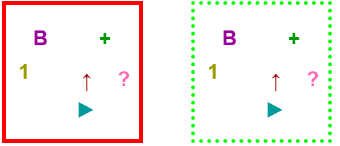
\includegraphics[scale=0.6]{Images/SelectionSeparadosIguales.png}
	\caption{An unselected element, to the left, is represented by solid red borders. The same element in a selected state, to the right, is indicated by dotted green borders.}
	\label{Figure:ElementSquares}
\end{center}
\end{figure}

If their selection  is  incorrect, the participant is shown which elements they misclassified (either by clicking them incorrectly or by failing to click them, see Figure~\ref{Figure:Misclassifications}). When they click a button to continue, they restart this stage (with a fresh randomization).

\begin{figure}[h!] 
\begin{center}
    	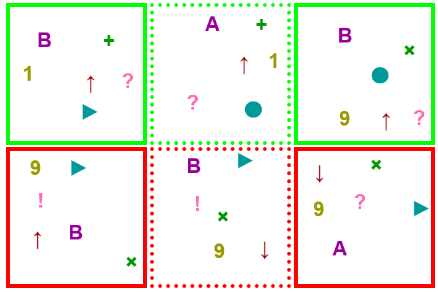
\includegraphics[scale=0.5]{Images/FeedBack2SeleccionParcial.PNG}
	\caption{A partial section of the feedback resulting from a wrong selection. A solid green border means that the box was correctly selected as belonging to the concept. A solid red border means that it was correctly left unselected, meaning that it did not belong to the concept. A dotted green border means the box belongs to the concept but was not selected, and a dotted red border means that the box does not belong to the concept but was selected.}
	\label{Figure:Misclassifications}
\end{center}
\end{figure}

When the participant finally makes the correct selection, they continue to the next phase. 

\subsubsection{The generalization phase}\label{Subsection:generalization}

In this phase, the participant is shown a subset of $U^i \backslash S^i$ (namely, in $(C^i_1 \cup C^i_2) \backslash (C^i_1 \cap C^i_2)$), that is, a selection of elements that were \emph{not} present in the learning phase (hence nor in the training phase). The participant must classify which of these elements they think belong to the concept. The participant does not receive feedback on the choices they make here. Except for the sixth trial, part of these elements satisfy the rule $\varphi^i_1 \land \lnot \varphi^i_2$, while the rest satisfy $\varphi^i_2 \land \lnot \varphi^i_1$. Thus \textemdash assuming the participant learned the concept via a process akin to a representation of one of the two rules\textemdash\, this phase crucially serves to distinguish which rule they have learned, if any.

After this selection, the participant is asked to submit a written explanation of what characteristics they think constitute the concept. This written explanation serves as an additional validation of whether they are thinking in a way describable by propositional logic according to our assumptions, or if rather they are using other methods (memorization, pen and paper, screenshots, other logics or formalisms, etc.). 


\subsection{Notes on the experiment design}\label{Experiment_design}

The elements, universes, and rules that constitute our experiment are devised in terms of propositional logic. However, it is important to be careful with the semantics, i.e.\ the way elements are actually shown to the participants. We have to avoid giving more salience to the semantics of a propositional variable over the others, and it is imperative to select the semantics of variables in a way such that they do not share characteristics that might escape our propositional grammar: for example, if the propositional variables were represented as circles that can be distinctly colored or not, it would be quite natural to assume that counting colored or uncolored circles could provide information, but this option is not considered in a theoretical design that assumes only propositional operators to describe rules. A related consideration is that we must also avoid introducing other regularities extraneous to the propositional formulation: if the images corresponding to all propositional variables are always shown in a straight line in the same order, salience effects might appear \textit{even if }we avoid semantics that become more expressive thanks to the ordered nature of the represented variables (such as with descriptions of the form \textit{the first and last elements are of the same size}).

\paragraph{Building adequate semantic representations for our logic.}
Taking these precautions into account, we choose to match each propositional variable with a particular image or figure, whose position in a square would be randomized (but avoiding superpositions). It  is harder to decide exactly what would be the matching, but our final decision consists in matching
each propositional variable with a set of two related Unicode characters (such as a triangle when the variable is $0$, and a circle otherwise). See Figure~\ref{Figure:references} for the exact representations. We take care to choose different types of characters for different variables: having $A,B$ for $\varA$ and $Y,Z$ for $\varE$ is out as a possibility, since it naturally  introduces counting of the type `there is no more than 1 letter' and the like.
Of course, this process is not fail-safe, as there are countless possible semantics associations that could introduce extra-propositional grammar into the experiment. But we try to minimize the chance that this happens easily or naturally, and we use the written explanation stage as a way to catch these exceptions if they occur\footnote{In the end, they did not occur. See \S\ref{Sec:ExclusionCriteria}.}. 

Finally, to minimize possible salience effects from showing symbols that could have (despite our intentions to the contrary) different levels of conspicuousness, we randomize on a per-participant basis the assignment between pairs of symbols and propositional variables (but we do not randomize  the assignment to the positive or negative value of a variable; the same Unicode characters  are  always positive in all randomizations, or always negative).

\paragraph{Ordering of positive and negative examples.}
As mentioned before, in the learning stage we shuffle the order in which their positive and negative examples are shown, but always presenting all positive examples first. Also, the number of positive examples is smaller or equal to the number of negative examples for all concepts (see Table \ref{trial_table}). 

The purpose of placing the positive examples first and having less positive examples than negative ones is to bias the participant into thinking of the concept by its positive formulation, instead of possibly thinking of a rule that would describe the negative examples, and then negating that rule to obtain the positive one. This becomes important when we want to reason about the ease of learning of different operators: the default assumption is that participants that correctly select positive examples of the concept are thinking the positive rule, which differs in its operator from the negative rule (by the De Morgan laws). 

